\documentclass[journal]{style/vgtc}           % final (journal style)
%\documentclass[review,journal]{style/vgtc}         % review (journal style)
%\documentclass[widereview]{style/vgtc}             % wide-spaced review
%\documentclass[preprint,journal]{style/vgtc}       % preprint (journal style)
%\documentclass[electronic,journal]{style/vgtc}     % electronic version, journal

%% Uncomment one of the lines above depending on where your paper is
%% in the conference process. ``review'' and ``widereview'' are for review
%% submission, ``preprint'' is for pre-publication, and the final version
%% doesn't use a specific qualifier. Further, ``electronic'' includes
%% hyperreferences for more convenient online viewing.

%% Please use one of the ``review'' options in combination with the
%% assigned online id (see below) ONLY if your paper uses a double blind
%% review process. Some conferences, like IEEE Vis and InfoVis, have NOT
%% in the past.

%% Please note that the use of figures other than the optional teaser is not permitted on the first page
%% of the journal version.  Figures should begin on the second page and be
%% in CMYK or Grey scale format, otherwise, colour shifting may occur
%% during the printing process.  Papers submitted with figures other than the optional teaser on the
%% first page will be refused.

%% These three lines bring in essential packages: ``mathptmx'' for Type 1
%% typefaces, ``graphicx'' for inclusion of EPS figures. and ``times''
%% for proper handling of the times font family.

\usepackage{mathptmx}
\usepackage{graphicx}
\usepackage{times}

%% We encourage the use of mathptmx for consistent usage of times font
%% throughout the proceedings. However, if you encounter conflicts
%% with other math-related packages, you may want to disable it.

%% This turns references into clickable hyperlinks.
\usepackage[bookmarks,backref=true,linkcolor=black]{hyperref} %,colorlinks
\hypersetup{
  pdfauthor = {},
  pdftitle = {},
  pdfsubject = {},
  pdfkeywords = {},
  colorlinks=true,
  linkcolor= black,
  citecolor= black,
  pageanchor=true,
  urlcolor = black,
  plainpages = false,
  linktocpage
}

%% If you are submitting a paper to a conference for review with a double
%% blind reviewing process, please replace the value ``0'' below with your
%% OnlineID. Otherwise, you may safely leave it at ``0''.
\onlineid{0}

%% declare the category of your paper, only shown in review mode
\vgtccategory{Research}

%% allow for this line if you want the electronic option to work properly
\vgtcinsertpkg

%% In preprint mode you may define your own headline.
%\preprinttext{To appear in an IEEE VGTC sponsored conference.}

%% Paper title.

\title{Interactive Visual Analysis of Image-Centric Cohort Study Data}

%% This is how authors are specified in the journal style

%% indicate IEEE Member or Student Member in form indicated below
\author{TBA}
\authorfooter{
%% insert punctuation at end of each item
\item
 Otto-v.-Guericke-University Magdeburg
}

%other entries to be set up for journal
\shortauthortitle{Klemm \MakeLowercase{\textit{et al.}}: Interactive Visual Analytics of Image-Centric Cohort Study Data}
%\shortauthortitle{Firstauthor \MakeLowercase{\textit{et al.}}: Paper Title}

%% Abstract section.
\abstract{Epidemiological population studies impose information about a set of subjects (a \emph{cohort}) to characterize disease specific risk factors.
%
Cohort studies comprise heterogenous data variables describing the medical condition as well as demographic and lifestyle factors of a subject.
%
Using well established statistical methods the data is hypothesis driven analyzed to find statistically significant variable correlations ('\emph{interactions}').
%
Modern cohort studies also incorporate medical image data.
%
Analyzing these data requires image segmentation, extraction of key figures and shape based subject grouping.
\\
We propose a Interactive Visual Analytics approach that enables epidemiologists to examine both image-based as well as sociodemographic and medical attribute data.
%We propose a Interactive Visual Analytics approach to provide epidemiologists with the tools necessary to analyze this data.
%
It allows for both classical hypothesis validation approaches as well as hypothesis generation by incorporating data mining methods.
%
Adaptive linked information visualization views and 3d-shape renderings are combined with epidemiological techniques.
%
Similarity measures between data variables are used to compute interesting changes in variable interactions for the current variable selection.
%
Shape based grouping of subjects is facilitated using hierarchical agglomerative clustering. (Remove Clustering reference?)
} % end of abstract


%% Keywords that describe your work. Will show as 'Index Terms' in journal
%% please capitalize first letter and insert punctuation after last keyword
\keywords{Interactive Visual Analytics, Epidemiology}

%% ACM Computing Classification System (CCS). 
%% See <http://www.acm.org/class/1998/> for details.
%% The ``\CCScat'' command takes four arguments.

\CCScatlist{ % not used in journal version
 \CCScat{K.6.1}{Management of Computing and Information Systems}%
{Project and People Management}{Life Cycle};
 \CCScat{K.7.m}{The Computing Profession}{Miscellaneous}{Ethics}
}

%% Uncomment below to include a teaser figure.
  % \teaser{
  % \centering
  % \includegraphics[width=16cm]{CypressView}
  % \caption{In the Clouds: Vancouver from Cypress Mountain.}
  % }

%% Uncomment below to disable the manuscript note
%\renewcommand{\manuscriptnotetxt}{}

%% Copyright space is enabled by default as required by guidelines.
%% It is disabled by the 'review' option or via the following command:
% \nocopyrightspace

%%%%%%%%%%%%%%%%%%%%%%%%%%%%%%%%%%%%%%%%%%%%%%%%%%%%%%%%%%%%%%%%
%%%%%%%%%%%%%%%%%%%%%% START OF THE PAPER %%%%%%%%%%%%%%%%%%%%%%
%%%%%%%%%%%%%%%%%%%%%%%%%%%%%%%%%%%%%%%%%%%%%%%%%%%%%%%%%%%%%%%%%

\begin{document}

%% The ``\maketitle'' command must be the first command after the
%% ``begin{document}'' command. It prepares and prints the title block.

%% the only exception to this rule is the \firstsection command
\firstsection{Introduction}

\maketitle

%% \section{Introduction} %for journal use above \firstsection{..} instead
Epidemiology aims to characterize health and disease by determining risk factors.
%
Clinical problems and questions answered using epidemiological methods comprise diagnosis accuracy, disease frequency, risk factors, disease prognosis, effectiveness of treatments or preventions and cause of diseases \cite{Fletcher2012}.
%
%Cohort studies are a epidemiological method to gather data about a group of subjects (a \emph{cohort)}) to make general statements about these problems.
%
Observations made by clinicians in the daily routine are translated into hypothesis.
%
These are used to determine environmental and lifestyle factors are as well as medical attributes which are believed to influence a condition of interest.
%
The data variables necessary are gathered using interviews and clinical examinations.
%
Statistical methods like regression analysis aim aim to check the attribute list for plausibility.
%

Longitudinal population-based studies like the Study of Health in Pomerania \cite{Volzke2011} aim to gather as much information as possible about a defined sample of people (a \emph{cohort}).
%
The sample is drawn randomized to avoid selection bias prohibit statements based on statistical correlations in the cohort to be inferred to the whole population (\emph{external validity}) \cite{Fletcher2012}.
%
Also a information bias needs to be avoided by strictly standardizing the data acquisition.
%
Statistical correlations are also prone to confounding, meaning that two factors influence each other and therefore should be normalized with respect to each other.
%
When for example one investigates risk factors for prostate cancer in male subjects the outcome is strongly dependent on the age.
%
Therefore results need to be age adjusted to be comparable.
%
Confounding variables, however, are often not obvious at all and characterizing them is already an epidemiological result.
\\\\
Modern cohort studies often include medical image data which introduces new problems.
%
Since it is unethical to expose people to radiation, non-harming imaging like Magnetic Resonance Imaging (MRI) or Ultrasound Imaging is used.
%
As MRI scans are expensive there exists a tradeoff between quality of the image data and their associated costs.
%
To quantify these data it is necessary to segment it.
%
Manual segmentation via radiological experts is possible but very costly and prone to inter- and intra observer variability.
%
Segmentation algorithms allow for (semi)-automated analysis of the data but require sophisticated methods due to high inter-subject variability caused by the subject diversity.
%
Analyzing spatial data with other epidemiological factors require techniques which reach beyond standard statistical methods.
\\
We propose a Interactive Visual Analysis approach \cite{Thomas2005} to provide a way to analyze both image- and non-image data.
%
Visual queries and direct feedback of Visual Analytics systems allow for a fast exploration of the data space.
%
Intended as a extension to the well established epidemiological tools it provides a way to rapidly validate hypothesis as well as trigger hypothesis generation using Data Mining methods such as clustering.
%
\textbf{ToDo Characterization of the healthy aging process! Which change indicates a unusual pathological change?}

%Interactive Visual Analysis (IVA) TODO QUELLE provides techniques which not only show promising potential for combining both 3d visualization with 

Our contributions are:
\begin{itemize}
	\item Applying the Interactive Visual Analysis approach to the epidemiological problem domain by characterizing special affordances of this context.
	\item Provide an overview over the workflow for analyzing cohort study data to gain insigth into the large subject spaces.
	\item Provide Visualization Techniques which combine both Information Visualization and 3D Rendering of Organ Shapes as well as combining them with well known epidemiological graphics and key figures.
	\item Implement the presented methods in a Web Framework based on WebGL, D3js and Nodejs as backend.
\end{itemize}

%Statistical correlations derived from analyzing the data itself may be misleading since 

%Include Implementation details - web based; how are image data included; what technologies are used?

\section{Medical and Technical Background} \label{MedicalAndTechnicalBackground}
Wer ist an epidemiologischen Studien beteiligt?\\
•  Ärzte (Facharzt für öffentliches Gesundheitswesen, Gene@ker)\\
•  Medizinische Informa@ker mit Fokus auf Biometrie und Sta@s@k\\
•  Bei klinischen Studien: Ärzte des entsprechenden Fachs

In this section we want to give insight into the epidemiological workflow when analyzing cohort study data to identify the problems we address in this paper.
%
ToDo Define Epidemiological Outcome
%
\subsection{Epidemiological Workflow} \label{EpidemiologicalWorkflow}
Epidemiologists follow a strict workflow mainly driven by statistic tools to validate hypothesis.
%
Following Thew and colleagues publication on this matter, the workflow can be characterized as follows.
%
Hypothesis most commonly base on observations made by clinicians in their daily routine.
%
A set of attributes depicting conditions affected by the hypothesis is compiled accordingly.
%
Confounding variables need to be adjusted so that they do not affect the effect size of a attribute.
%
Statistical methods such as regression analysis are applied to measure the effect size of attributes to the outcome of interest.
%

Reproducibility of results is an epidemiological key requirement.
%
Longitudinal epidemiological studies require the acquired attributes to be comparable to evaluate them.
%
If the data acquisition process changes, a information bias is introduced to the data, disallowing inference between acquisition cycles.
%
This underlines the high quality standards to methods processing the data, whether to extract additional parameters or gain insight.
%
To determine, whether a subject is prone to be affected by a certain disease, relative risks a expressed through the evaluation of p values which indicate statistical significance.
%
Statistics tools such as SPSS and STATA play a major role for analyzing epidemiolgical data. 
%
Graphic data representation is largely used to show results rather than gaining insight.
\\
Group subjects using epidemiological factors is essential in order to make statements about their statitical power.
%
Grouping is carried out hypothesis driven.
%
Age for example is also divided into groups (\emph{binned}) when investigating its influence on a condition.
%
These groups depend strongly on the condition of interest and therefore there is no defined standard on how to categorize these values.
	
\subsection{Epidemiological Data} \label{EpidemiologicalData}
Epidemiological data is highly heterogenous.
%
Information about medical history and examinations, genetic conditions, geographical data, questionaire answers, and image data yield complex data spaces for each subject.
%
Often data are derived from acquired variables to either group or threshold values or get information derived from reviewed data such as breast density data for women.
%
This underlines also the problem of missing data since for ethical, legal or medical reasons some data variables can not be gathered for each subject.
%
Follow-up examinations or -questions for conditions also produce variables only available for a small amount of subjects.
%

Indicators for medical conditions as well as questions about a subjects lifestyle are also often \emph{dichotomous}, meaning that they only have two manifestations (often \emph{Yes} or \emph{No}).
%
This allows for the calculation of \emph{odds ratios} which describe the relation of two \emph{dichotomous} variables, allowing for direct comparison of their influences.
%
Dichotomous data can also be derived by combining aggregating data variables to yield only two manifestations (e.g. subjects younger or older than 50).
%

\paragraph{Image acquisition.} \label{ImageAcquisition} Imaging techniques emitting an hazardous amount of radiation for the subject are not suited for ethical reasons.
%
MRI data is more expensive to obtain as CT data but does not affect the subjects health and is therefore the main method for collecting cohort study imaging data.
%
The quality of medical image data acquired for cohort studies is a tradeoff between accuracy and affordability \cite{Preim2014}.
%
This often yields image resolutions inferior to those of clinical day-to-day practice, which makes their analysis more challenging.

\paragraph{Image analysis.} \label{ImageAnalysis} When analyzing medical image data there have decisions to be made on how they are \emph{compared} and \emph{quantified}.
%
Segmentations masks describing all parts of the shape of interest would be ideal since many different key figures can be derived from them.
%
Since these masks require sophisticated algorithms custom tailored to the data sets the epidemiologists are forced to measure the data by hand, which is a very tedious work with respect to the number of necessary landmarks and number of subjects.
%
Information derived by landmarks are also not nearly as expressive and versatile as segmentation masks.
%
They are also prone to a high inter-observer variability and hard to reproduce.
%
This gains even more momentum when analyzing multiple time steps!
%
Morphometric information from landmarks comprises thickness, diameter or length of a structure as well as grey-value distribution in an area (used for determine type of tissue).

% Bernhard Paper\\
% - sociodemographic data\\
% - medical data\\
% - pain indicators\\
% - DATA TYPES\\
% 	- dichotomous data\\
% \\
% - Missing Data\\
% - Follow-Up Questions?\\
% - grouping essential\\
% - problems when analyzing image data\\
% 	- what are Problems there\\
% 	- how can shape be included?\\
% 	- show image data of multiple subjects


\subsection{The Study of Health in Pomerania (SHIP)}
Starting 1997 with a cohort consisting of 4.308 subjects this cohort study located in northern Germany aims to characterize health and disease in the widest range possible \cite{Volzke2011}.
%
Data is collected independent of diseases in mind.
%
This allows the data set to be queried regarding many different diseases and conditions.
%
Subjects were examined in a 5-year time span, continuously adding new parameters including MRI scans in the last iteration of 2012.
%
The MRI protocol features a rich number of different sequences.
%
Also for women, breast MRI scans were acquired.
%
A second cohort \texttt{SHIP-Trend} was established in 2008 to acquire data about a younger population.
%
The protocols for analyzing the subjects between \texttt{SHIP} and \texttt{SHIP-Trend} remained the same, making them comparable.
%
The overall examination time for each person attending the study is two days.

\section{Prior and Related Work}
Einfuehren von Helwigs Terminologie?

Finding a visualization which fits all needs and communicates all aspects of the data equally is challenging.
%
Given the number of features of epidemiological data sets and their different manifestations, it is often a good solution to combine the strength of different visualization techniques in a unified system \cite{Buja91, Konyha2009}
%
Data mining tools like the Principal Component Analysis are able to reduce the dimension by extracting most expressive components, but making the influence of each variable hard to determine.
\\\\
The work of Turkay and colleagues is closest to ours albeit our focus on processing medical image data and variables with categorical manifestations \cite{Turkay2013}.
%
Investigating Data on an norwegian aging study their methods aim to amplify a hypothesis generation process when analyzing the data.
%
Statistical measures of metric variables such as mean, standard deviation, skewness, or inter-quartile range are used to create \emph{dimension plots}.
%
These transform dimensions into data points and make them comparable with respect to the derived descriptive measures.
%
This not only allows for comparing all continuous variables in a single plot but make their distribution change comprehensible.
%
This of course requires a good descriptive measure which captures the kind of change the user is interested in or which reflects unexpected data behavior.
%
The technique was applied to variables generated by segmenting the the brain into 45 parts and measure the number of voxel, volume and properties of the intensity values.
%
The method is strongly dependent on the descriptive derived measures of the epidemiological factors.
%
Hypothesis based on observations of changes in these plots may impose over-fitting to the data because the measure highlights certain statistical changes.
%
Our approach sticks more to the information extracted from the segmented image data and derive variable interaction with non-image epidemiological factors.
% Disadvantage - Nur 2 abgeleitete Variablen sichtbar, schlecht mit anderen Variablen in Verbindung zu bekommen (müsste jedoch auch gehen) - viele Dinge gehen durch die Abstraktion aber auch flöten!

Gresh and colleagues suggest with \texttt{WEAVE} one of the first systems which analyzed medical image and non-image data using linked views \cite{Gresh2000}.
%
Blaas and colleagues presented a similar system which analyzed medical image data and variables derived from them using views from the feature- and physical space \cite{Blaas2007}.
%
This approach already incorporated Data Mining approaches like dividing the data space using a k-nearest-neighbor technique and Principal Component Analysis.
%
Steenwijk and colleagues employ a relational database to organize the data to visualize subject data using linked views like parallel coordinates, scatterplots and time plots \cite{Steenwijk2010}.
%
Zhang and colleagues provide a web-based system for analyzing subject groups with linked views and batch-processing capabilities for categorizing new subject entries into the data set \cite{Zhang2012}.
%
Their understanding of a cohort differs from the understanding of the term in an epidemiolgical context.

Commercial systems like Tableau or Spotfire provide a rich user interface that allows to apply Visual Analytics techniques without the need of writing any code.
%
With little efford linked views can be created using these tools, but the data procesinng possibilities like derivation of new variables or the volume rendering capabilities are very limited.
%
These systems share limitations in extensibility to a specific problem domain.
%Spotfire offers the possibilities to interact with the \texttt{R} statistical programming language 

% *********************** Our own Work ***********************
Klemm and colleagues used captured lumbar spine variabilities based on an semi-automatic shape-detection algorithm of 490 participants of the \texttt{SHIP-2} \cite{Klemm2013VMV}.
%
Hierarchical agglomerative clustering was used to divide the population into shape-related groups.
%
As proof of concept a relation between size of the segmented shape and measured size of the subjects was measured and behaved as expected.
%
This work focuses on incorporating these data as new features of the overall data set, making it possible to include it into the hypothesis validation and generation process.
%
When applying clustering techniques on the non-image data is was found that \texttt{k-Prototypes} and \texttt{DBSCAN} is appropriate in the epidemiological context but is strongly dependent on the chosen variables and distance measure \cite{Klemm2014BVM}.
% *********************** / Our own Work ***********************

Generalized Pairs Plot (\emph{GPLOMS}) is an information visualization technique that allows for heterogenous variables to be pairwise visualized using appropriate plots in a plot matrix grouped by type.
%
This technique is also useful to gain an overview over numerous variables and their distributions.
%
It uses histograms, bar charts, scatterplots and heat maps to visualize the different variable combinations with regard to their type.
%
Brushing capabilities allow for brushing and linking as well as filtering, but has limitations like making only one category brushable at a time.
%
We applied this technique to our data and it shows promising potential for simultaneously visualizing many different variable but does not fit in the scope of this paper.
%
A similar approach was taken by Dai and colleagues for risk factor exploration as they also incorporate choropleth maps of epidemiological factors (e.g. mortality rates in a region) with parallel coordinates, bar charts and scatterplots integrated regression lines \cite{Dai2005}.
%
From their findings regarding the interaction of cancer-related socio-demographic factors are drawn in a \emph{Concept Map} where related factors are connected via graph-edges.

Chui and colleagues visualized interactions in time-dependant epidemiological data using time-series plots highlighting risk factors differences in age and gender \cite{Chui2011}.
%
\\\\
% Image Data
Comparing tissue between many subjects in an epidemiological context requires methods which allow for shape variance visualizations.
%
Caban and colleagues investigated the suitability of variance visualizations of shape distribution models and concluded in their user study that user favor spherical glyph representations over deformation grids and likelihood volumes \cite{Caban2011}.
%
The distribution of shapes in a space derived from a principal component analysis is plotted by Busking and Colleagues in a 2D-projected plane of the space \cite{Busking2010a}.
%
We incorporate the idea of combining 3D-Shape rendering with information visualization techniques.
%
Differences between structures are highlighted using color mapping of the difference to the mean shape, but is rather hard to recognize due to small renderings of each subject in the shape-space.
%
Via mesh morphing interpolated views can be created by the user in a separate view as well as comparisons in contour-view.
%
Applying our data sets to this technique yielded a cluttered shape space due to the many subjects.
%
The data needs to abstracted or summarized in order to work in this context.
%
In order to detect local deformation changes, Hermann and colleagues investigating shape related difference by letting the user specify a deformation of interest and showing corresponding changes in the shape using covariance tensors \cite{Hermann2014}.
%
This method allowed for rapid hypothesis validation and was able to reproduce textbook knowledge.
%
By plotting p-values in ventricle surfaces, Chou and colleagues were able to map disease-associated values directly on a 3D tissue representations \cite{Chou2009}.
%
This requires a geographic colocation of associated features.
%

% Interactive Visual Analysis - Steffens Paper
The strength of the Interactive Visual Analysis approach described in the next section is it's versatility with respect to the application field \cite{Konyha2009}.
%
Oeltze and colleagues combined a linked view representation of results from a statistical analysis with feature localizations of the human blood flow with the goal of its evaluation \cite{Oeltze2007}.
%
%They aim to provide methods to analyze perfusion data with respect to 
While we take similar steps when analyzing the data like employing statistical tests, our data is mostly independent from the medical image data and is not describing it--except the variables derived the segmentation model itself.

\section{Interactive Visual Analytics in Cohort Study Data}
\begin{figure}[htb]
 \centering
 \label{fig:WorkflowComparison}
 %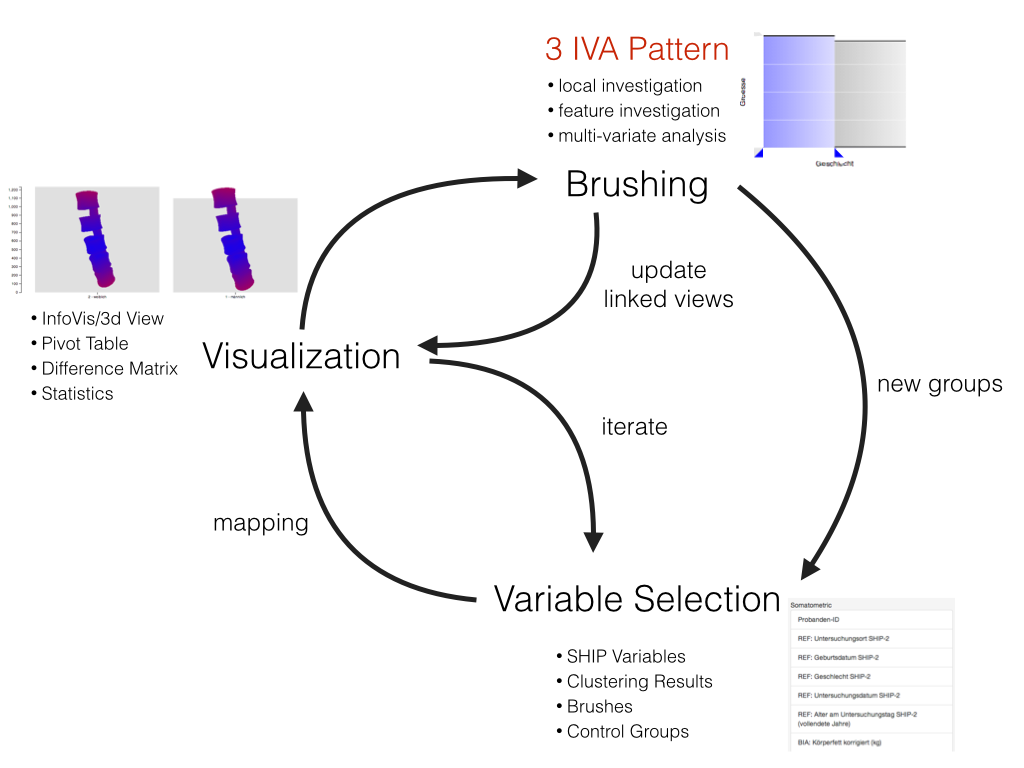
\includegraphics[width=1.5in]{figures/InteractionLoop}
 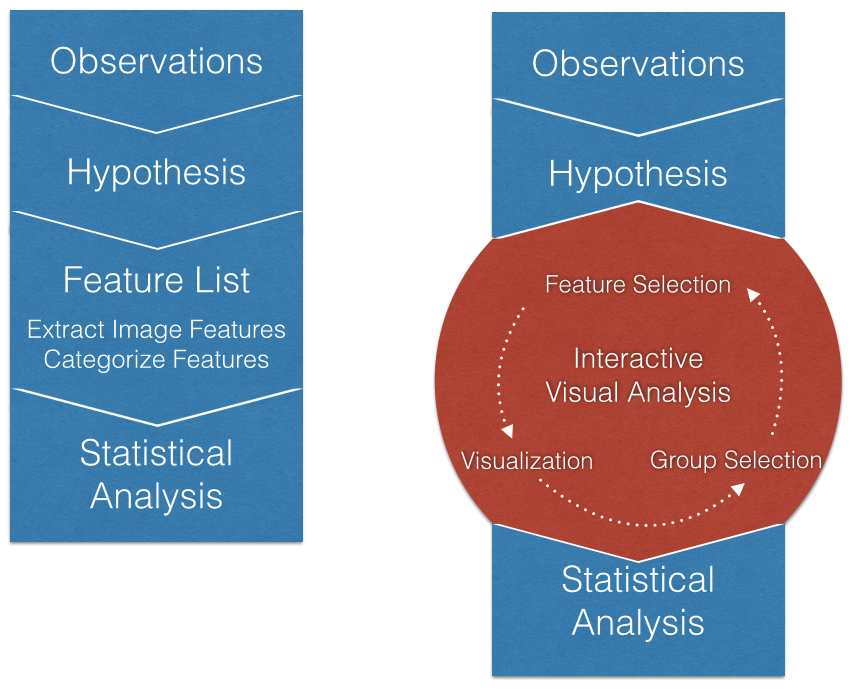
\includegraphics[width=3.0in]{figures/workflow_comparison}
 \caption{Visual Analytics systems are able to complement parts of the epidemiological workflow, not to replace it. The appropriate combination of statistical- and interactive driven analysis shows promising potential to unveil the information in the data.}
\end{figure}
\begin{figure}[htb]
 \centering
 %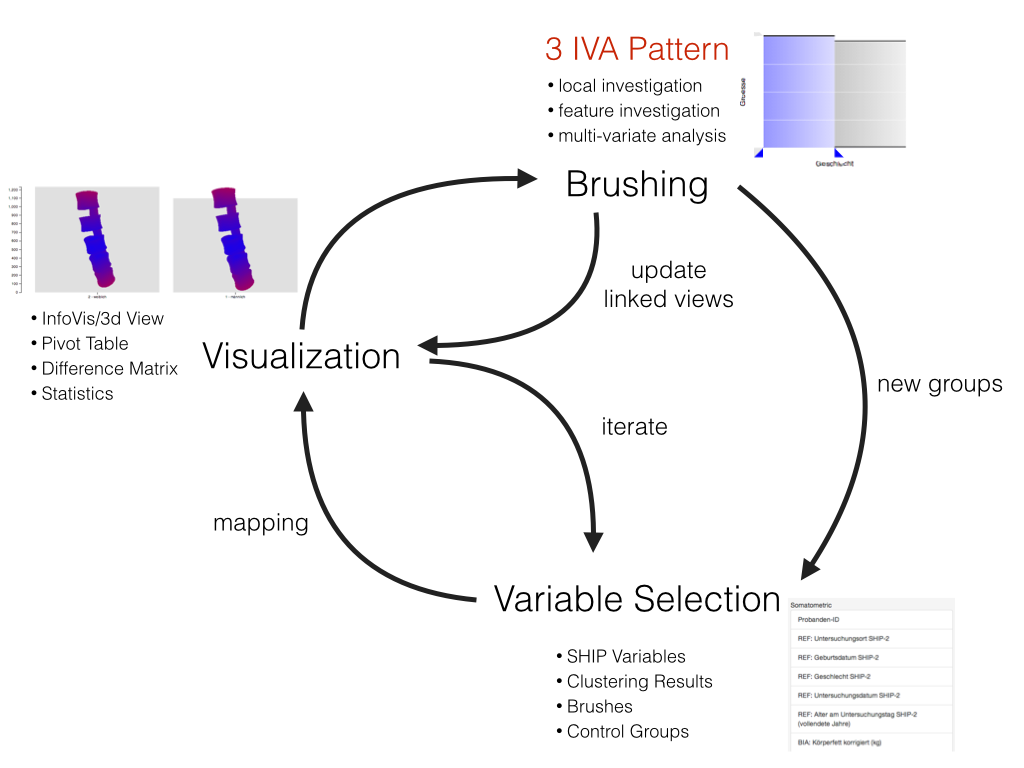
\includegraphics[width=1.5in]{figures/InteractionLoop}
 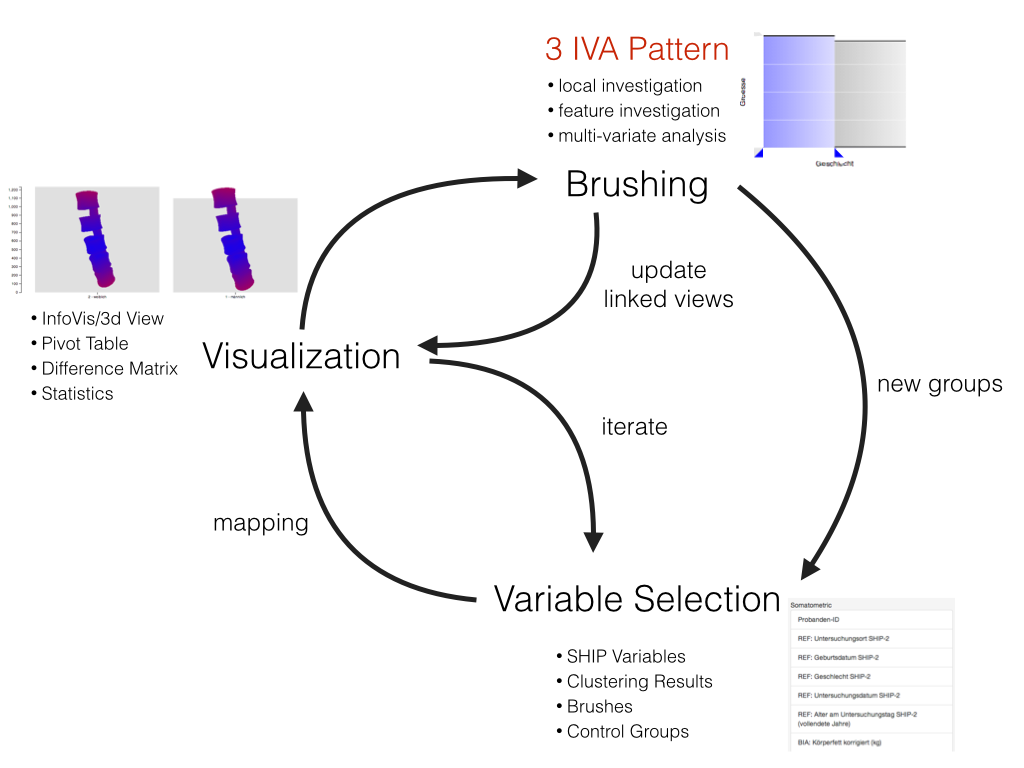
\includegraphics[width=3.0in]{figures/InteractionLoop}
 \caption{Interaction Overview}
\end{figure}

As described in subsection~\ref{EpidemiologicalWorkflow}, the epidemiolgical workflow is a strict sequence of steps taken by domain experts and needs to be reproducible and comprise statistical integrity.
%
Figure~\ref{fig:WorkflowComparison} (a) describes this workflow as steps consecutive series of steps.
%
The workflow we propose by introducing the \emph{IVA} principle into the epidemiological problem domain does not aim to replace the existing workflow but to complement its weaknesses 
%
In the current state the workflow handles the data as a black box.
%
A list of features describing the hypothesis is compiled and analyzed using statistical tests. 
%
The resulting value decides whether the data supports the hypothesis or not.
%
It would be possible that there actually are features of the data set which support the hypothesis by discriminating the population in the expected way, but with this approach it is not able to find those.
%
This becomes even more imminent when the workflow is adapted to the analysis of the medical image data.
%
Domain experts annotate tediously landmarks which allow to derive metrics like distances which are then handled like other features and analyzed using the same set of statistical tools.
%
Not only does this leave out the majority of the information in the medical image data by abstracting it to metrics, it is easily possible that information left out would heavily influence the result.
%
Considering more complex parts of the data would make those results more trustworthy and also could identify possible anatomical confounders--an epidemiolgical research result in itself.
%
Statistical tests check for validity of the number but not for their completeness or plausibility!
\\\\
IVA tries to illuminate the data black box by making the domain experts part of the feature list selection process.
%
Figure~\ref{fig:WorkflowComparison} (b) highlights the iterative process as part of the epidemiolgical workflow.
%
Note that the process also aims to project back into the hypothesis formulation step to amplify hypothesis generation 
%
This has to be handled with care since overfitting of expectations to the available data is an imminent danger as described by Turkay and colleagues \cite{Turkay2013}.

According to Steffens Terminology in Interactive Visual Analysis of Perfusion Data
\\\\
\textbf{Object Space}\\
- Medical Image Data / Spine Segmentations\\
\textbf{Attribute Space}\\
- SHIP-Variables\\
- Derived visualizations

? Where to incorporate Levels of IVA

\subsection{Feature Selection}
- Automatic using Clustering\\
- Automatic using Statistical Recommendations\\
- Via User Input

\subsection{Brushing the information space} 
- derive new groups which serve as input for the feature selection

\subsubsection{Feature Localization}
- Projection from Image Space to Attribute data. This is more difficult in our application, because we currently only brush on derived features.\\
- Clustering in Image Space yields Groups which can be analyzed using the attribute space\\
- Create a Pipeline Overview over different Levels of different IVA Patterns and Stages

\subsubsection{Local Investigation}
- Selection of Information using Bar Charts, Scatterplots or Parallel Coordinates which projects the selection into the Object space\\
- this selection is for categorical data already given implicitly bei projecting the 3D-View onto the Bar Charts/Mosaik Plots!\\
- this aims to locale features of the data!\\
- Gain Information about SHIP-Variables by putting them into the context of each other. The Pivot Table allows for direct numerical\\ analysis, while the information visualizations allow for better insight of the combination

\subsubsection{Multivariate Analysis}
- Selection of Elements in Scatterplots, Barcharts or Parallel Coordinates Views - observe how selection changes another view - this allows for multivariate analysis\\
- Becker, R.A., Cleveland, W.S.: Brushing scatterplots. Technometrics 29(2) (1987)\\
- Wang Baldonado, M.Q., Woodruff, A., Kuchinsky, A.: Guidelines for using multiple views in information visualization. In: AVI ’00: Proceedings of the working conference on Ad- vanced visual interfaces, pp. 110–119. ACM Press, New York, NY, USA (2000). DOI\\ http://doi.acm.org/10.1145/345513.345271
- By brushing individual parameters or create new binnings of parameter it is possible to see how they change in coordinated views. This is already implemented in the Cargo framework\\
- by creating comparative 3d Visualizations it is possible to assess the influence of non-image parameters to the visual space.

\subsection{Implementation}
Diagram of used Technologies

\section{Application}

\subsection{The Spine Dataset}
- Describe steps from gathering Information from the raw image files (segmentation, abstraction, visualization)\\
- Input of Epidemiologists goes here!\\
\\\\
\textbf{From VMV'13 Paper}\\

All whole-body MRI scans were acquired on a 1.5~Tesla scanner (Magnetom Avanto; Siemens Medical Solutions, Erlangen, Germany) by four trained technicians in a standardized way. Subjects were placed in the supine position. Five phased-array surface coils were placed to the head, neck, abdomen, pelvis, and lower extremities for whole-body imaging. The spine coil is embedded in the patient table. The spine protocol consisted of a sagittal T1-weighted turbo-spin-echo sequence (676 / 12 [repetition time msec / echo time msec]; 150$^\circ$ flip angle; 500~mm field of view; $1.1\times1.1\times4.0~mm$ voxels) and a sagittal T2-weighted turbo-spin-echo sequence (3760 / 106 [repetition time msec / echo time msec]; 180$^\circ$ flip angle; 500~mm field of view; $1.1\times1.1\times4.0~mm$ voxels). First, both sequences were placed over the cervical and upper thoracic spine. Then, they were placed over the lower thoracic and lumbar spine. The MRI software automatically composed a whole spine sequence from the two T1-weighted and T2-weighted sequences \cite{Hegenscheid2013}. We were provided with 490 data sets.

%The model is placed in the scene using an empirically chosen initialization point. The force acting on the model stems from aggregation of loads, which are derived from a potential field resulting from a weighted sum of the T1- and T2-weighted MRI images, see \cite{Rak2013}. After detecting all spines, we register the models because in a later clustering step we only want to capture the local deformation of the lumbar spine, not different locations in world space. The models are registered using the Kabsch Algorithm \cite{Kabsch1976}, which is designed to minimize the root mean squared deviation between paired sets of points.
The model is placed in the scene using an empirically chosen initialization point. The force acting on the model stems from aggregation of loads, which are derived from a potential field resulting from a weighted sum of the T1- and T2-weighted MRI images, see \cite{Rak2013}. After detecting all spines, we register the models because in a later clustering step we only want to capture the local deformation of the lumbar spine, not different locations in world space. The models are registered using the Kabsch Algorithm, which is designed to minimize the root mean squared deviation between paired sets of points.
The model-based detection captures information about the spine canal curvature as well as the alignment of the vertebrae. It is not meant to capture information about vertebrae deformation and differences in spine canal extent.

\section{Summary and Conclusion}

%% if specified like this the section will be committed in review mode
%\acknowledgments{SHIP is part of the Community Medicine Research net of the University of Greifswald, Germany, which is funded by the Federal Ministry of Education and Research (grant no. 03ZIK012), the Ministry of Cultural Affairs as well as the Social Ministry of the Federal State of Mecklenburg-West Pomerania. Whole-body MR imaging was supported by a joint grant from Siemens Healthcare, Erlangen, Germany and the Federal State of Mecklenburg-Vorpommern. The University of Greifswald is a member of the ‘Centre of Knowledge Interchange’ program of the Siemens AG. This work was supported by the DFG Priority Program 1335: Scalable Visual Analytics.}

\bibliographystyle{abbrv}
%%use following if all content of bibtex file should be shown
%\nocite{*}
\bibliography{bibliography}
\end{document}
